\documentclass{article}
\usepackage[utf8]{inputenc}
\textheight = 25cm 
\textwidth = 15cm
\topmargin = -3.0cm 
\oddsidemargin = 1.5cm
\usepackage{hyperref}
\hypersetup{
    colorlinks=true,
    linkcolor=blue,
    filecolor=blue,
    citecolor=black,      
    urlcolor=blue,
    }

\usepackage{float}
\usepackage{graphicx}

\usepackage{gensymb}

\usepackage{amsmath}
\usepackage{amssymb}
\usepackage{amsfonts}
\usepackage{mathtools, xparse}
\usepackage[shortlabels]{enumitem}

\usepackage[many]{tcolorbox}
\usepackage{lipsum}

\title{Tarea 2 Termodinámica}
\author{Cerritos Lira Carlos, Calderon Alba Sebastian}
\date{3 de abril del 2020}

\begin{document}
\maketitle
\section*{1.-}
Considerando que la energía interna de un sistema hidrostático es una función de $T$ y $p$, 
deducir las ecuaciones:
\begin{enumerate}[a)]
    \item \[ dQ 
    = \left[ \left( \frac{\partial U}{\partial T}\right)_p + p\left( \frac{\partial V}{\partial T} \right)_p \right] dT
    + \left[ \left(\frac{\partial U }{\partial p}\right)_T + p\left( \frac{\partial V}{\partial p} \right)_T \right] dp \]
    \item \[ \left(\frac{\partial U}{\partial T}\right)_p 
    = C_p - pV\beta \]
    \item \[ \left( \frac{\partial U}{\partial p}\right)_T 
    = pVk_T - (C_p-C_V)\frac{k_T}{\beta} \]
\end{enumerate}
\begin{tcolorbox}[breakable]
    
\end{tcolorbox}

\section*{2.-}
Un líquido se agita irregularmente en un recipiente bien aislado y por ello experimenta 
una elevación de temperatura. Considerando el líquid como sistema:
\begin{enumerate}[a)]
    \item ¿Ha habido una transferencia de calor? 
    \item ¿Se ha realizado trabajo?
    \item ¿Cuál es el signo de $\Delta U$?
\end{enumerate}
\begin{tcolorbox}[breakable]
    
\end{tcolorbox}

\section*{3.-} 
Un mol de gas ideal monoatómico está confinado en un cilíndro con un pistón, y se mantiene 
a temperatura constante $T_0$ dentro de un baño térmico. El gas lentamente se expande de
$V_1$ a $V_2$ mientras se sigue manteniendo a temperatura $T_0$. ¿Por qué la energía interna 
del gas no cambia?. Calcular el trabajo hecho por el gas y el calor que fluye hacia el gas.
\begin{tcolorbox}[breakable]
    
\end{tcolorbox}

\section*{4.-}
En la expansión adiabática de un gas ideal se cumple $PV^{\gamma} = cte$. Mostrar que también 
se vale:
\begin{align*}
    TV^{\gamma -1} &= cte \\
    T &= cte p^{1-\frac{1}{\gamma}}
\end{align*}
\begin{tcolorbox}[breakable]
    
\end{tcolorbox}
\section*{5.-}
Explicar las contribuciones energéticas para cada proceso en el ciclo de Otto, que se 
recorre en el sentido $a \to b \to d \to a$. Calcular la eficiencia del ciclo.
\begin{figure}[H]
    \centering
    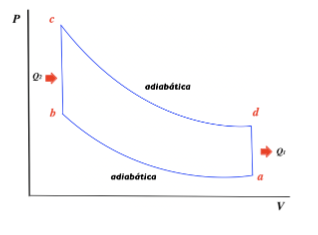
\includegraphics{images/p5_cycle.png}
\end{figure}
\begin{tcolorbox}[breakable]
    
\end{tcolorbox}

\end{document}